\subsection{Расстояние и размеры}
\textit{Параллакс} --- изменение видимого положения объекта относительно удалённого фона в зависимости от положения наблюдателя.
\begin{equation}r=\frac{1}{\pi}
\end{equation}
Где $r$ --- расстояние до звезды (в парсеках), $\pi$ --- годовой параллакс звезды (в секундах).
\begin{figure}[!h]
\centering
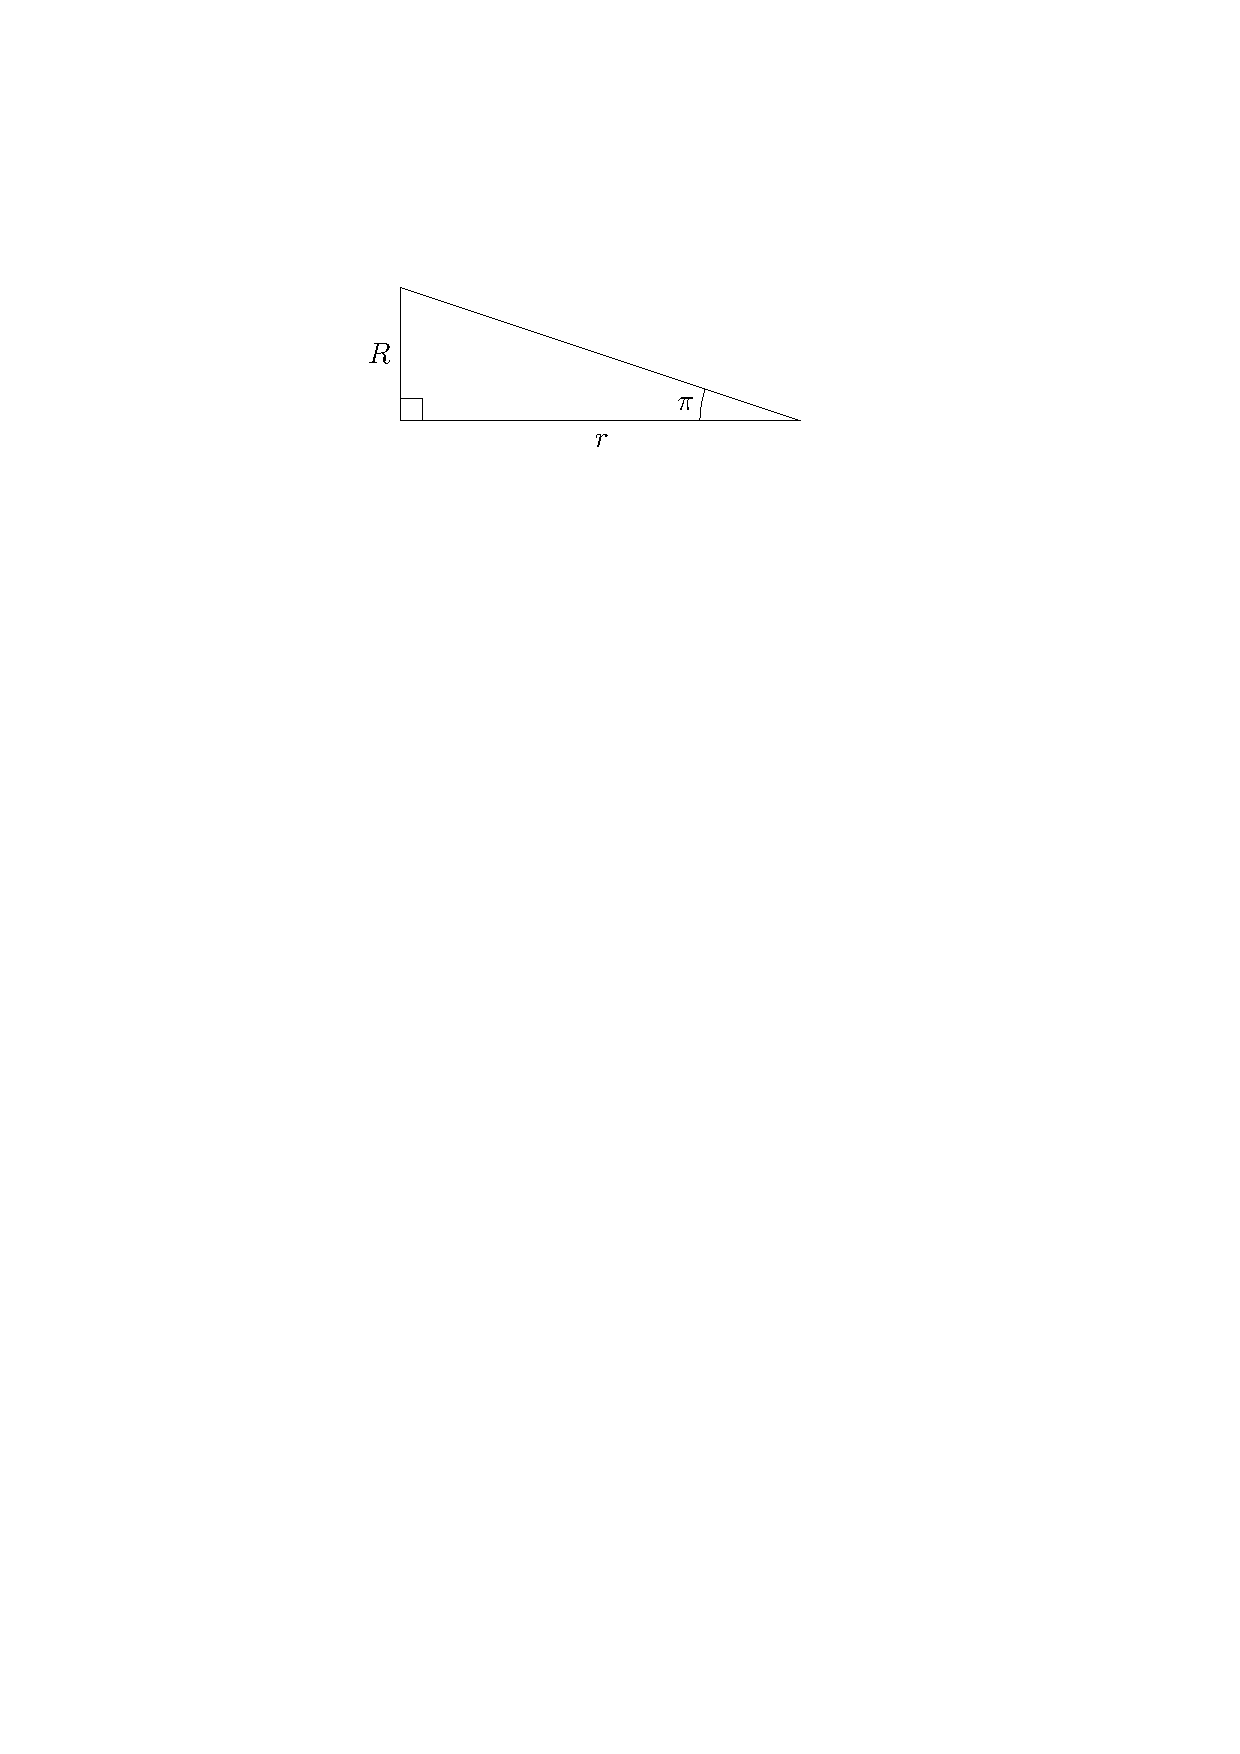
\includegraphics[width = 0.37\textwidth]{1-second}
\caption{Параллакс в одну секунду}
\end{figure}

Если $R$ --- радиус орбиты Земли, $r$ --- расстояние до объекта, $\pi$ --- годовой параллакс, то параллакс будет равен $\pi=1''$ с расстояния $r=1$пк.
$$\sin\pi_{\text{рад}}\approx\pi_{\text{рад}}=\frac{R}{r}=\frac{1\text{ а.е.}}{206265\text{ а.е.}}\Rightarrow\pi_{\text{сек}}\cdot 206265''\frac{1\text{ а.е.}}{206265\text{ а.е.}}\Rightarrow\pi_{\text{сек}}=\frac{1\text{ а.е.}}{1\text{ пк}}$$

\textit{Горизонтальный параллакс} --- параллакс светила при положении последнего на горизонте.
\begin{equation}r=\frac{R_{\text{З}}}{\sin p_0}=\frac{3438'}{p_0'}R_{\text{З}}=\frac{206265''}{p_0''}R_{\text{З}}
\end{equation}
Где $R_{\text{З}}$ --- радиус Земли, $p_0$ --- горизонтальный экваториальный параллакс.

\textbf{Правило Тициуса-Боде} --- эмпирическая формула приблизительно описывающая радиусы орбит планет от Солнца:
\begin{equation}r=\frac{3\cdot 2^n+4}{10}
\end{equation}
Где $n=-\infty, 0, 1, 2...$

Расстояние, радиус и угловой размер объекта соотносятся следующим образом:
\begin{equation}R=r\frac{\rho'}{3238'}=r\frac{\rho''}{206265''}
\end{equation}
Где $R$ --- радиус объекта, $\rho$ --- угловые размеры объекта. $\sin\rho\approx\rho$ (приближение для малых углов).
